\section{Auswertung}

\subsection{Vergleichswerte}

Vor der Durchführung des Experiments werden folgende Werte für den Vergleich mit den zu bestimmenden Werten aufgenommen:

\begin{align*}
    Abstand Detektor-Spalt \; \;  L &= 1.05m \\
    Spaltbreite (Einzelspalt)\; \; b_e &= 0.15*10^{-3}m \\
    Spaltbreite (Doppelspalt)\; \; b_d &= 0.15*10^{-3}m \\
    Spaltabstand\; \; s &= 0.5*10^{-3}m \\
    Dunkelstrom\; \; I_{Dunkel} &= 1*10^{-8}A\\
    Wellenlaenge Laserlicht\; \; \lambda &= 633*10^{-9}m 
\end{align*}

\subsection{Einzelspalt}

Die Werte für die Messung am Einzelspalt sind in Tabelle \ref{tab:1} zu finden.

\begin{minipage}{\linewidth}
    \begin{table}[H]
        \centering
    \captionof{table}{Messwerte für die Beugung am Einzelspalt}
    \begin{tabular}{ll}
        \toprule
        x-$x_0$ [mm] & I [mA] \\
        \midrule
        -20  &   0.0025 \\ 
        -19  &   0.0015 \\ 
        -18  &   0.0020  \\ 
        -17  &   0.0030  \\ 
        -16  &   0.0040  \\ 
        -15  &   0.0020  \\ 
        -14  &   0.0015 \\ 
        -13  &   0.0050  \\ 
        -12  &   0.0070  \\ 
        -11  &   0.0055 \\ 
        -10  &   0.0025 \\ 
        -9   &   0.0070  \\ 
        -8   &   0.0125 \\ 
        -7   &   0.0145 \\ 
        -6   &   0.0080  \\ 
        -5   &   0.0075 \\ 
        -4   &   0.0285 \\ 
        -3.5 &   0.1600   \\ 
        -3   &   0.2400   \\ 
        -2.5 &   0.3200   \\ 
        -2   &   0.4000    \\ 
        -1.5 &   0.4500   \\ 
        -1   &   0.4600   \\ 
        -0.5 &   0.4500   \\ 
        0.5  &   0.2800   \\ 
        1    &   0.2000    \\ 
        1.5  &   0.1200   \\ 
        2    &   0.0640  \\ 
        2.5  &   0.0230  \\ 
        3    &   0.0060  \\ 
        3.5  &   0.0025 \\ 
        4    &   0.0070  \\ 
        5    &   0.0110  \\ 
        6    &   0.0090  \\ 
        7    &   0.0035 \\ 
        8    &   0.0035 \\ 
        9    &   0.0070  \\ 
        10   &   0.0070  \\ 
        11   &   0.0040  \\ 
        12   &   0.0015 \\ 
        13   &   0.0025 \\ 
        14   &   0.0040  \\ 
        15   &   0.0020  \\ 
        16   &   0.0005 \\ 
        17   &   0.0015 \\ 
        18   &   0.0030  \\ 
        19   &   0.0025 \\ 
        20   &   0.0010  \\ 
        \bottomrule   
    \end{tabular}
    
    \label{tab:1}
\end{table}
\end{minipage}

Von den Werten für die Intensität wird der Dunkelstrom abgezogen. Anschließend werden die entstehenden Werte graphisch dargestellt. Dabei wird auf der x-Achse der Beugungswinkel $\phi$ dargestellt. Dieser berechnet sich ungefähr durch $\phi = \frac{x-x_0}{L}$. Es wird eine Ausgleichsrechnung mit folgender Formel durchgeführt:

\begin{align*}
    I=A_0^2\cdot b^2\cdot (\dfrac{\lambda}{\pi \ b \ \sin{\psi}})^2 \cdot \sin{\pi \ b \ (\sin{\dfrac{\phi}{\lambda}}})^2.
\end{align*}

Dabei entsteht das Folgende Diagramm:

\begin{figure}[H]
    \centering
    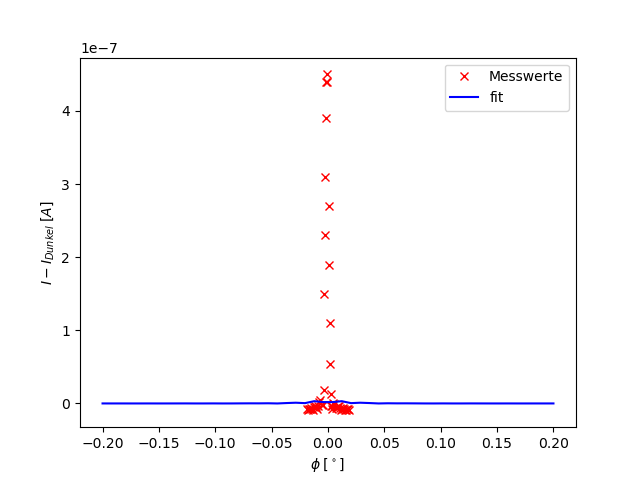
\includegraphics{einzel.png}
    \captionof{figure}{Beugung des Laserlichts am Einzelspalt mit Ausgleichsrechnung.}
\end{figure}

Diese Ausgleichsrechnung liefert nun einen Wert für die Breite des Spaltes:

\begin{align*}
    b = (0.146\pm 0.000127)*10^{-3}m
\end{align*}

\subsection{Doppelspalt}

Die Werte für die Beugung am Doppelspalt sind in Tabelle \ref{tab:2}.

\begin{minipage}{\linewidth}
    \begin{table}[H]
        \centering
    \captionof{table}{Messwerte für die Beugung am Doppelspalt}
    \begin{tabular}{ll}
        \toprule
        x-$x_0$ [mm] & I [mA] \\
        \midrule
        -20  &   0.0020 \\ 
        -19  &   0.0040 \\ 
        -18  &   0.0110  \\ 
        -17  &   0.0095  \\ 
        -16  &   0.0020   \\ 
        -15  &   0.0045  \\ 
        -14  &   0.0150 \\ 
        -13  &   0.0130  \\ 
        -12  &   0.0040  \\ 
        -11  &   0.0060 \\ 
        -10  &   0.0210 \\ 
        -9   &   0.0180  \\ 
        -8   &   0.0050 \\ 
        -7   &   0.0120 \\ 
        -6   &   0.1600  \\ 
        -5   &   0.2000 \\ 
        -4   &   0.0200 \\ 
        -3.5 &   0.0150   \\ 
        -3   &   0.0230   \\ 
        -2.5 &   0.5000   \\ 
        -2   &   1.0000    \\ 
        -1.5 &   0.3000   \\ 
        -1   &   3.0000   \\ 
        -0.5 &   1.4000   \\ 
        0.5  &   5.0000   \\ 
        1    &   0.6000    \\ 
        1.5  &   2.5000   \\ 
        2    &   2.5000  \\ 
        2.5  &   0.1300 \\ 
        3    &   1.0000  \\ 
        3.5  &   0.2800 \\ 
        4    &   0.0500  \\ 
        5    &   0.0125  \\ 
        6    &   0.1300  \\ 
        7    &   0.0900 \\ 
        8    &   0.0050 \\ 
        9    &   0.0030  \\ 
        10   &   0.0180  \\ 
        11   &   0.0180  \\ 
        12   &   0.0045 \\ 
        13   &   0.0040 \\ 
        14   &   0.0120  \\ 
        15   &   0.0120  \\ 
        16   &   0.0025 \\ 
        17   &   0.0025 \\ 
        18   &   0.0080  \\ 
        19   &   0.0080 \\ 
        20   &   0.0200    \\ 
        \bottomrule   
    \end{tabular}
    
    \label{tab:2}
\end{table}
\end{minipage}

Für die graphische Darstellung dieser Werte wird genau so vorgegangen wie bei den Werten für den Einzelspalt. Diesmal wird die Ausgleichsrechnung allerdings mit folgender Formel durchgeführt: 

\begin{align*}
    I= A_0^2\cdot \cos{\dfrac{\pi\ s \sin{\phi}}{\lambda}}^2 \cdot
    (\dfrac{\lambda}{\pi \ b \sin{\phi}})^2 \cdot (\sin{\dfrac{\pi\ b \sin{\phi}}{\lambda}})^2.
\end{align*}

Dabei entsteht folgendes Diagramm

\begin{figure}[H]
    \centering
    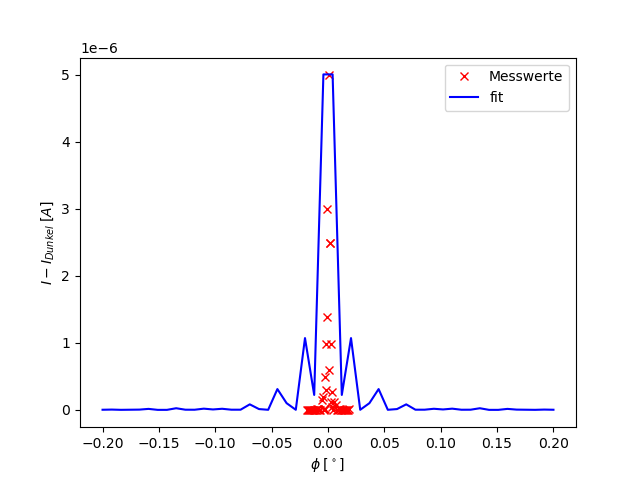
\includegraphics{doppel.png}
    \captionof{figure}{Beugung des Laserlichts am Doppelspalt mit Ausgleichsrechnung.}
\end{figure}

Die Ausgleichsrechnung liefert dabei einen Wert für die Spaltbreite und den Spaltabstand:

\begin{align*}
    b &= (0.1335\pm 0.0001)* 10^{-3}m \\
    s &= (0.659\pm 0.000195)* 10^{-3}m  
\end{align*}

\subsection{Vergleich}

Beim Vergleich der beiden Kurven entsteht das Bild in Abbildung \ref{fig:Vergleich}.

\begin{figure}[H]
    \centering
    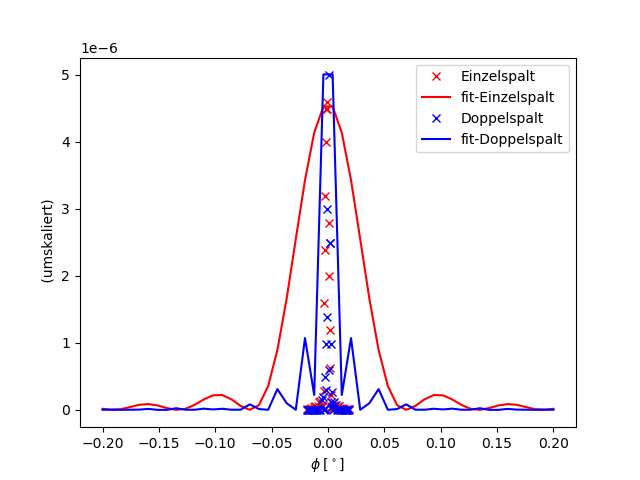
\includegraphics{vergleich.png}
    \captionof{figure}{Vergleich der Beugungsmessungen.}
    \label{fig:Vergleich}
\end{figure}


\section{Diskussion}

Das Experiment liefert die Werte

\begin{align*}
    b_e = (0.146\pm 0.000127)*10^{-3}m \\
    b_d = (0.1335\pm 0.0001)* 10^{-3}m  \\
    s = (0.659\pm 0.000195)* 10^{-3}m.
\end{align*}

Die theoretischen Werte sind

\begin{align*}
    b_e = 0.15*10^{-3}m \\
    b_d = 0.15* 10^{-3}m  \\
    s = 0.5* 10^{-3}m.
\end{align*}

Die durch die Ausgleichsrechnungen entstehenden Werte werden mit den angegebenen Werten verglichen. 

\begin{equation*}
    \Delta \% = \frac{x_{Theo}-x_{Exp}}{x_{Theo}}
\end{equation*}

Dabei entstehen folgende Abweichungen:

\begin{align*}
b_e \; \; & \text{weicht um} \; \; 2.67\% \; \; \text{ab} \\
b_d \; \; & \text{weicht um} \; \; 11.00\% \; \; \text{ab} \\ 
s \; \; & \text{weicht um} \; \; 31.8\% \; \; \text{ab}  \\
\end{align*}

Dieses Experiment hat einige Fehlerquellen. Diese sind zum Beispiel die Ausrichtung des Lasers und des Detektors. Diese werden vor der messung per Hand und mit bloßem Auge ausgerichtet. Es ist also äußerst wahrscheinlich das bereits hierbei kleinere fehler entstanden sind.

Da die Messwerte von einem analogen Messgerät abgelesen werden ist die während des Experiments herrschende Dunkelheit ein Faktor der einen ohnehin schon vorhandenen Fehler beim Ablesen noch vergrößert. Denn eine Lichtquelle zum Ablesen der Werte würde die Messung der Intensität beeinflussen.

Die Dunkelheit liefert allerdings eine weitere Ungenauigkeit. Denn es ist nicht möglich den Raum vollständig abzudunkeln. Dies würde widerum auch ein ablesen der Werte völlig unmöglich machen. Zwar wurde diese Ungenauigkeit versucht mit dem Dunkelstrom wieder auszugleichen jedoch war es dadurch, dass dieser so klein ist auch sehr schwer seinen genauen Wert zu bestimmen.

Das Messgerät selbst lieferte auch eine zusätzliche Fehlerquelle. Nämlich hat das Wechseln der Messbereiche zu leichten Veränderungen der Werte geführt. Um den Fehler dabei zu minimieren wurde so gut wie möglich versucht den Messbereich beizubehalten, dies war aufgrund von großen Schwankungen der Werte nicht immer möglich.

Weiterhin gab es die Fehlerquelle, dass die Spalte eingeklemmt werden mussten. Dies geschah per Hand und daher ist auch hier Fehler zu erwarten. Es war weder gegeben, dass der Spalt genau gerade ausgerichtet war, noch das der Laser genau mittig durch die Spalte schien und außerdem besteht durch eine starke Abnutzung der Klemmvorrichtung auch die Möglichkeit, dass die Spalte leicht verrutscht sind.

Die Ausgleichsrechnungen sind hier auch eine Fehlerquelle, die Auflösung der Minima und Maxima ist durch die begrenzte Anzahl an Messwerten klein. Es wurden zwar 50 Messwerte genommen aber gerade in der Nähe des Hauptmaximums wären noch mehr werte nötig gewesen um noch bessere Ausgleichsrechnungen zu erhalten.

Zuletzt sei noch zu dem Vergleich des Beugungsbilds vom Einzelspalt mit dem vom Doppelspalt gesagt, dass, wie in der Abbildung zu erkennen, bis auf einige Ausnahmen die Kurve für den Einzelspalt, die Einhüllende für die Kurve des Doppelspaltes darstellt.